\subsection{定位、轨迹与导航算法}
\subsubsection{已知地图方法的建图与定位分离}
方式二在障碍物布置完成后建图，再在固定地图上定位和导航。仓库与课程环境使用 gmapping 建图、\texttt{map\_\allowbreak server} 加载地图、AMCL 估计本车地图位姿、\texttt{move\_\allowbreak base} 完成路径与速度规划。建图和比赛运行阶段要分开；gmapping 与 AMCL 不应同时发布相同 map→odom 变换，否则 TF 来源竞争会使导航位姿不一致。

gmapping 的原理背景参见~\cite{gmapping}。gmapping 背后的 Rao-Blackwellized 粒子滤波将轨迹和地图联合后验分解：每个粒子表示机器人轨迹假设，并持有相应地图。激光扫描匹配和里程计先验影响粒子权重，回环处尤其需要足够视角和合理运动。照片里的低纹理板面不妨碍几何扫描，但相似长直通道可能让定位沿通道方向约束较弱；开放端和转角更利于区别位置。

实验地图必须连同 yaml 和 pgm 保存，并记录分辨率、原点和障碍布置版本。仓库 slam/maps 的 room1/room2 属参考资料，不能当作这张照片场地的比赛地图。照片拓扑图也不能转换为虚构 gmapping 输出。比赛现场修改围挡、移动横板或缩小通道后应重新测绘建图，避免规划器在旧空闲区撞上新增实体。
\begin{equation}
p(x_{1:t},m\mid z_{1:t},u_{1:t})=p(m\mid x_{1:t},z_{1:t})\,p(x_{1:t}\mid z_{1:t},u_{1:t})
\end{equation}
\par 场地拓扑见图~\ref{fig:route}。
\begin{table}[H]\centering\small
\begin{tabularx}{\linewidth}{p{27mm}X}\toprule
核对项 & 技术含义与参数\\\midrule
准备阶段 & 驱动 + 传感器 + gmapping + \texttt{map\_\allowbreak saver}\\
比赛阶段 & \texttt{map\_\allowbreak server} + AMCL + \texttt{move\_\allowbreak base}\\
地图证据 & 实测 pgm/yaml、分辨率、原点、布置版本\\
\bottomrule\end{tabularx}
\caption{已知地图方法的建图与定位分离的实现要点。}\end{table}

建图结果、定位输入与导航调用需要绑定同一张地图及坐标约定。地图文件存在并不保证 AMCL 已收敛，首次运行仍应通过实际扫描与地图的重合关系确认初始位姿。

\source{\path{README.md}；\path{maps/README.md}；\path{slam/README.md}。版本以本报告提交号及配置快照为准。}
\subsubsection{AMCL 粒子定位与协方差有效性}
AMCL 在已知地图中递归估计机器人位姿，运动模型预测粒子，观测模型以扫描与地图一致性更新权重，再进行自适应采样。定位不是一次初始位姿输入后永久有效；若机器人被搬起、里程计异常或扫描缺失，后验可能变宽或跳到错误通道。Follower.\texttt{on\_\allowbreak loc} 使用 \texttt{frame\_\allowbreak id} 和协方差对定位输入作初步质量检查。

\texttt{localization\_\allowbreak ok} 检查 36 元协方差数组中 x、y、yaw 的对角元素，要求有限、非负并低于配置上限。地图 follower 默认 x/y 上限 0.25、yaw 上限 0.35，量纲分别为 m\(^{2}\) 和 rad\(^{2}\)，不是位置/角度误差本身。协方差小也不等于位置正确，多峰分布、错误初值或观测模型过度自信可能产生低协方差误定位。

AMCL 在静止时不一定持续发布新位姿；仓库 \texttt{localization\_\allowbreak refresh} 定期请求无运动更新，并要求有效扫描。该机制更新观测证据，不允许凭服务请求制造假的新定位。验证需要检查扫描更新时间、AMCL 新时间戳及 map 到 base 的连通性；定位失效后重新初始化并记录重置，不应让后车依据过期位置持续追踪。
\begin{equation}
w_t^{(i)}\propto p(z_t\mid x_t^{(i)},m)w_{t-1}^{(i)},\quad \Sigma_{xx},\Sigma_{yy}\le0.25,\quad\Sigma_{\psi\psi}\le0.35
\end{equation}
\par 坐标链由共享 map 与各车独立 odom/base 组成。
\begin{table}[H]\centering\small
\begin{tabularx}{\linewidth}{p{27mm}X}\toprule
核对项 & 技术含义与参数\\\midrule
协方差检查 & 数组长度 36；有限；非负；对角阈值\\
静止更新 & \texttt{request\_\allowbreak nomotion\_\allowbreak update} + 新扫描支持\\
额外验证 & 真实位姿误差、重定位稳定性、TF 连通\\
\bottomrule\end{tabularx}
\caption{AMCL 粒子定位与协方差有效性的实现要点。}\end{table}

协方差门限提供的是定位有效性筛选，并不直接保证真实位姿误差小于某个距离。环境重复或地图失配时仍可能产生错误匹配，因此需结合扫描对齐、TF 连续性和时间戳共同判断。

\source{\path{turtlebot/follow2/multi_robot_following/src/competition_core/planning.py}；\path{turtlebot/follow2/multi_robot_following/scripts/localization_refresh.py}。版本以本报告提交号及配置快照为准。}
\subsubsection{目标测量、地图变换与轨迹缓存}
方式二的领航目标可来自 TonyPi AR 标记或前车共享地图位姿。\texttt{marker\_\allowbreak target} 把观测按测量时间转换到地图；\texttt{pose\_\allowbreak relay} 校验前车位姿。\texttt{map\_\allowbreak follower} 只接受地图坐标系正确、新鲜、严格递增时间戳且跳变可接受的目标。没有目标时不会从 TonyPi 的动作次数生成地图位置，这避免把开环步数误当作准确领航里程计。

Trail 用有界折线保存测得目标位置，默认 spacing=0.08 m、\texttt{max\_\allowbreak length}=20 m、\texttt{jump\_\allowbreak limit}=0.8 m。相邻目标变化小于采样间距时保留旧点以降低噪声和存储；跳变超过上限被拒绝，目标时间戳不会因此刷新。总弧长超限时删除前端旧点，保证长时间运行不会无限增长。默认参数是设计起始值，其大小必须与真实目标运动速度和更新间隔相容。

对弯道，弧长缓存保留路径转角，而单纯按领航机器人瞬时朝向后退可能把目标放到墙内。必须进一步说明：保留转角的目标点不等于机器人严格复现轨迹，\texttt{move\_\allowbreak base} 仍可能在可通行区域平滑或改变局部路径。想证明无切角，应比较后车实际轨迹到领航折线的距离，而不是只画目标点。
\begin{equation}
\ell_k=\|p_k-p_{k-1}\|,\qquad L=\sum_k\ell_k,\qquad p_k\text{接受条件：}\ell_k\le \ell_{\mathrm{jump}}
\end{equation}
\begin{figure}[H]\centering
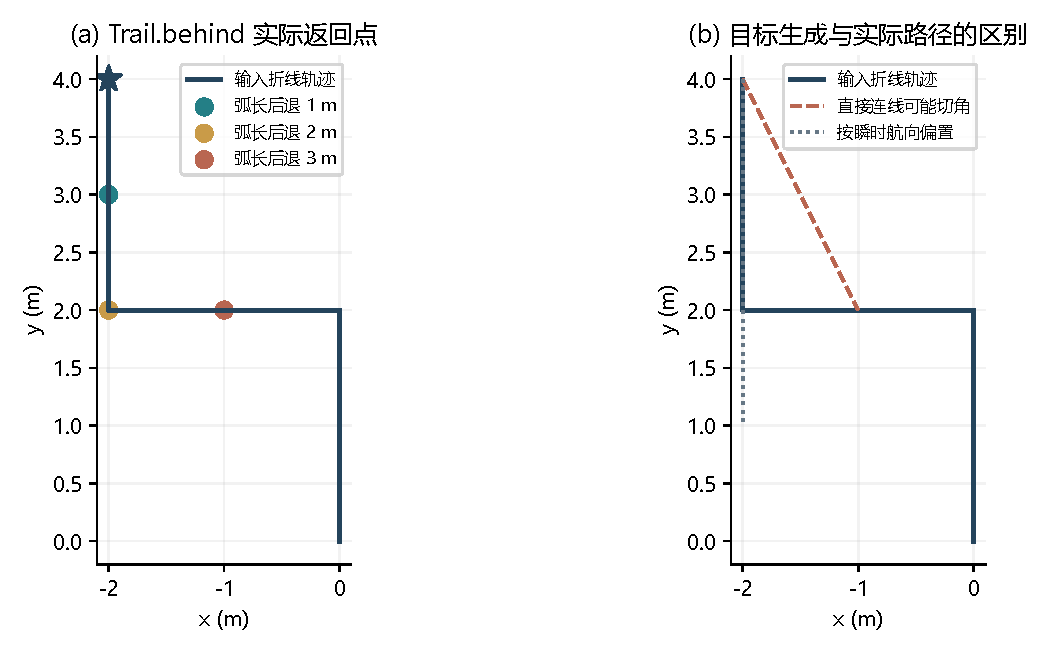
\includegraphics[width=.96\linewidth,height=85mm,keepaspectratio]{figures/analysis/trail.pdf}
\caption{核心 Trail.behind 对合成折线的真实返回值。输入点以米为单位，仅用于解释弧长算法。}\label{fig:f2a-trail}
\end{figure}

不同回退距离对应同一折线上的不同位置，结果取决于累计路程和末段插值。输入历史过短时，回退目标不能凭空延伸到未知路径，跟随器必须结合最小轨迹长度与间距条件决定是否发出目标。下面将这些条件与采样参数一并列出，便于复核配置。

\begin{table}[H]\centering\small
\begin{tabularx}{\linewidth}{p{27mm}X}\toprule
核对项 & 技术含义与参数\\\midrule
有效来源 & 带时间戳 AR 变换 / 共 map 前车位姿\\
采样约束 & 0.08 m 间距；0.8 m 跳变上限；20 m 缓存\\
导航边界 & 目标沿折线；实际路径由规划器决定\\
\bottomrule\end{tabularx}
\caption{目标测量、地图变换与轨迹缓存的实现要点。}\end{table}

采样时刻决定目标应使用哪一个相机位姿进行变换；弧长参数决定沿缓存轨迹回退多远。将这两类参数混为纯位置偏移会在转弯和运动中引入系统误差，因此日志应同时记录时间戳、地图点和轨迹长度。

\source{\path{turtlebot/follow2/multi_robot_following/src/competition_core/planning.py}；\path{turtlebot/follow2/multi_robot_following/scripts/map_follower.py}。版本以本报告提交号及配置快照为准。}
\subsubsection{全局路径规划、障碍膨胀与未知区域}
地图导航先在栅格代价地图中选择可行目标，再由全局规划器连接本车与目标。实体围挡、扫描障碍和机器人足迹共同确定可行性。围挡照片中的通道较窄，膨胀半径越大，规划越偏向通道中心，但过度膨胀可能让本可通过的通道没有可行目标；减小膨胀必须以实测轮廓和定位误差为依据，不能只为了让路径出现。

\texttt{grid\_\allowbreak clear} 采用圆形足迹并考虑单元格面积，检查半径加上半个栅格对角线范围内所有单元。未知值小于零或占据值达到阈值均视为阻塞，越界和无效地图也拒绝目标。地图 follower 默认阈值 65，RGB-D Grid.clear 默认阈值 95，二者对 OccupancyGrid 的保守性不同；这些值不能和内部 costmap 的 0—255 代价直接互换。

目标点可行只证明该点周围足迹没有被当前地图占据，不证明从当前位置存在完整路径；规划器仍需处理连通性和局部动态障碍。全局地图应保留固定围挡，动态扫描进入局部及全局障碍层。对于传感器未看到的区域，保守未知处理可能让机器人等待，这是信息不足的结果，不应通过将 NaN 深度标成自由空间解决。
\begin{equation}
r_{\mathrm{check}}=r_{\mathrm{robot}}+\frac{\sqrt2}{2}\,s,\qquad c_i<0\ \text{或}\ c_i\ge c_{\mathrm{th}}\Rightarrow\mathrm{blocked}
\end{equation}
\begin{figure}[H]\centering
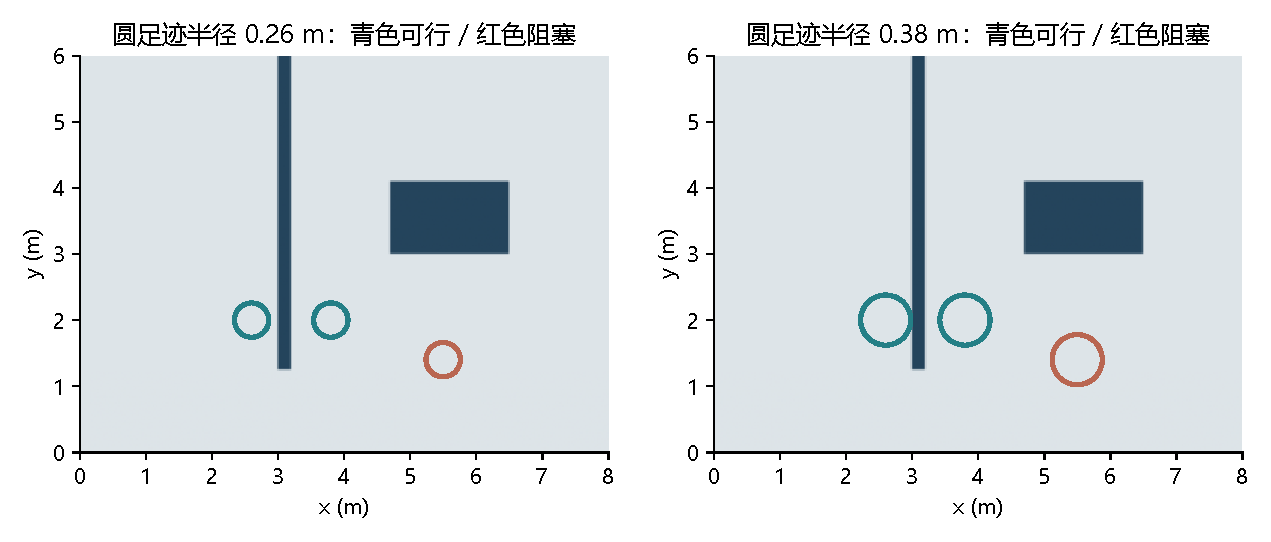
\includegraphics[width=.96\linewidth,height=85mm,keepaspectratio]{figures/analysis/footprint.pdf}
\caption{圆足迹、栅格离散化和未知区域的安全检查示例，使用实际 \texttt{grid\_\allowbreak clear} 函数判断颜色。}\label{fig:f2a-footprint}
\end{figure}

足迹检查把候选目标由单个点扩展为具有车体半径的区域；中心格可通行不代表整个机器人可放入。栅格边界补偿用于降低离散采样遗漏风险，未知区域则按不可进入处理。表中列出检查时涉及的地图量纲与边界约束。

\begin{table}[H]\centering\small
\begin{tabularx}{\linewidth}{p{27mm}X}\toprule
核对项 & 技术含义与参数\\\midrule
单元量纲 & OccupancyGrid：-1 未知、0—100 占据值\\
足迹补偿 & 半径 + 半栅格对角线\\
可行层级 & 目标局部足迹可行与整条路径连通分开\\
\bottomrule\end{tabularx}
\caption{全局路径规划、障碍膨胀与未知区域的实现要点。}\end{table}

足迹检查负责筛除不可放置的候选目标，规划器负责寻找可连接的路径，二者互不替代。即使目标点通过检查，也可能因通道过窄或地图连通性问题无法规划；这类失败需要保留导航状态与对应栅格。

\source{\path{turtlebot/follow2/multi_robot_following/src/competition_core/planning.py}；\path{turtlebot/follow2/multi_robot_following/config/costmap_common.yaml}。版本以本报告提交号及配置快照为准。}
\subsubsection{DWA 速度采样、动力学与弯道通行}
DWA 的原始方法参见~\cite{dwa}，本工程使用 ROS 配置中的实现。局部规划器 DWA 在满足速度及加速度限制的窗口中采样线速度和角速度，对短时轨迹作代价评价。地图配置以 10 个线速度样本、20 个角速度样本和 1 个横向样本工作，最大线速 0.15 m/s、最大角速 0.5 rad/s；RGB-D 配置采用 12×25 样本和更低 0.12 m/s、0.4 rad/s 上限。轨迹展开图展示采样候选的几何差异，不是调用完整 ROS DWA 得到的获胜轨迹。

差速底盘不能横向平移，因此曲线来自 v、\(\omega\) 的组合。路径距离权重偏向全局路线，目标距离权重鼓励接近目标，障碍代价限制靠近围挡；权重改变通常会影响在狭窄弯道的犹豫、贴墙或局部振荡。\texttt{sim\_\allowbreak time} 较长可以看见更远的碰撞，却会增加计算并把未来不确定性带入选择。运动采样必须与实际制动能力一致。

仓库关闭恢复旋转和 \texttt{clearing\_\allowbreak rotation\_\allowbreak allowed}，以免失去目标后后台旋转继续运动。导航 ABORTED、REJECTED 或 LOST 会锁定故障，排查后重启 follower。这个配置选择牺牲部分自主逃离能力，换取目标保持和受控恢复；实测比较应记录等待时间、导航失败和人工重置，而不能只计算最终到达率。
\begin{equation}
\dot x=v\cos\psi,\quad\dot y=v\sin\psi,\quad\dot\psi=\omega,\qquad J=w_pJ_p+w_gJ_g+w_oJ_o
\end{equation}
\begin{figure}[H]\centering
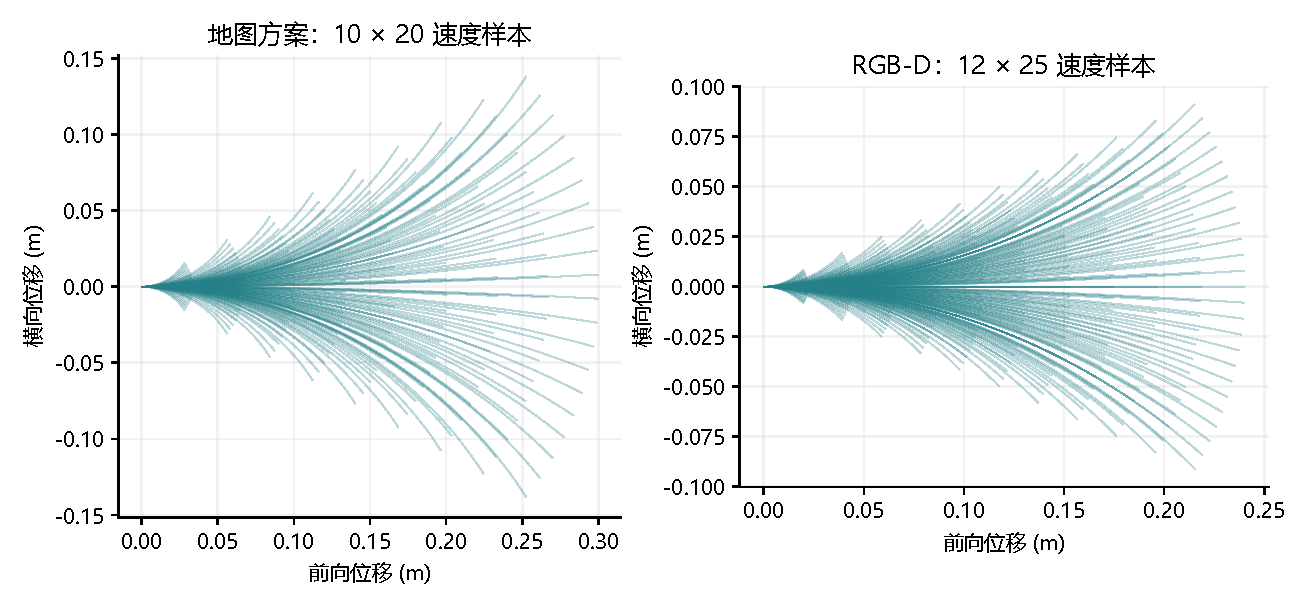
\includegraphics[width=.96\linewidth,height=85mm,keepaspectratio]{figures/analysis/dwa.pdf}
\caption{按配置速度范围展开的运动学候选轨迹。图未调用 ROS 局部规划器评分，属于采样几何演示。}\label{fig:f2a-dwa}
\end{figure}

候选轨迹展示速度与角速度组合如何改变短时运动范围，而实际选择还取决于障碍代价、路径距离和目标距离评分。图中没有运行这些评分项，不能用曲线数量或形状推断避障成功率。配置核对应进一步确认采样密度、预测时域与制动能力是否匹配。

\begin{table}[H]\centering\small
\begin{tabularx}{\linewidth}{p{27mm}X}\toprule
核对项 & 技术含义与参数\\\midrule
地图方案 & max v=0.15；max \(\omega\)=0.5；10×20 样本\\
RGB-D 方案 & max v=0.12；max \(\omega\)=0.4；12×25 样本\\
恢复行为 & 禁用旋转恢复；失败锁定并请求排故\\
\bottomrule\end{tabularx}
\caption{DWA 速度采样、动力学与弯道通行的实现要点。}\end{table}

表中两套配置分别约束地图方案与 RGB-D 方案的候选运动，不能把更密的采样直接解释为更高成功率。减小速度上限可降低短时位移，却也改变弯道跟随和超时行为；禁用旋转恢复后，受阻可能需要人工复位。实际调参应同时记录通道宽度、局部障碍和导航失败状态。

\source{\path{turtlebot/follow2/multi_robot_following/config/move_base.yaml}；\path{turtlebot/follow3/rgbd_following/config/navigation.yaml}。版本以本报告提交号及配置快照为准。}
\subsubsection{导航目标更新、取消与停止不变量}
移动目标持续变化，若每帧向 \texttt{move\_\allowbreak base} 发送新目标，规划容易不断抢占并产生振荡。\texttt{map\_\allowbreak follower} 使用 \texttt{goal\_\allowbreak interval} 和 \texttt{goal\_\allowbreak shift} 双阈值，默认至少间隔 1 s 且目标移动 0.25 m 才重发；首次目标无条件发送。该滤波位于目标发布层，不能替代感知关联，也不能掩盖真实的突然变向。

RGB-D \texttt{need\_\allowbreak goal} 使用 0.5 s 间隔、普通位移阈值 0.15 m，并对最终目标或成功状态将位移阈值降到 0.02 m，防止到终点时微小目标更新被忽略。相同“限频”概念在两套代码中实现不同，报告应分别列出参数，不能把最终目标修正能力泛化到地图 follower。地图版本保留了较简单的完成判断，需在终点试验中检查其旧目标冻结风险。

任何不满足许可的 step 调用 block，撤销 \texttt{motion\_\allowbreak allowed} 并取消已有 goal。导航状态 4、5、9 会锁定 failed，后续循环不再自动恢复。停止不是删除当前状态信息：\texttt{follow\_\allowbreak status} 保留明确原因，便于区分 \texttt{target\_\allowbreak lost}、\texttt{leader\_\allowbreak too\_\allowbreak close}、costmap stale 和 localization invalid。这样的可观察停车行为是系统诊断的重要组成部分。
\begin{equation}
\mathrm{Resend}=\bigl(\Delta t\ge\tau_g\bigr)\land\bigl(\|g_t-g_{t^-}\|\ge\epsilon_g\bigr)
\end{equation}
\begin{figure}[H]\centering
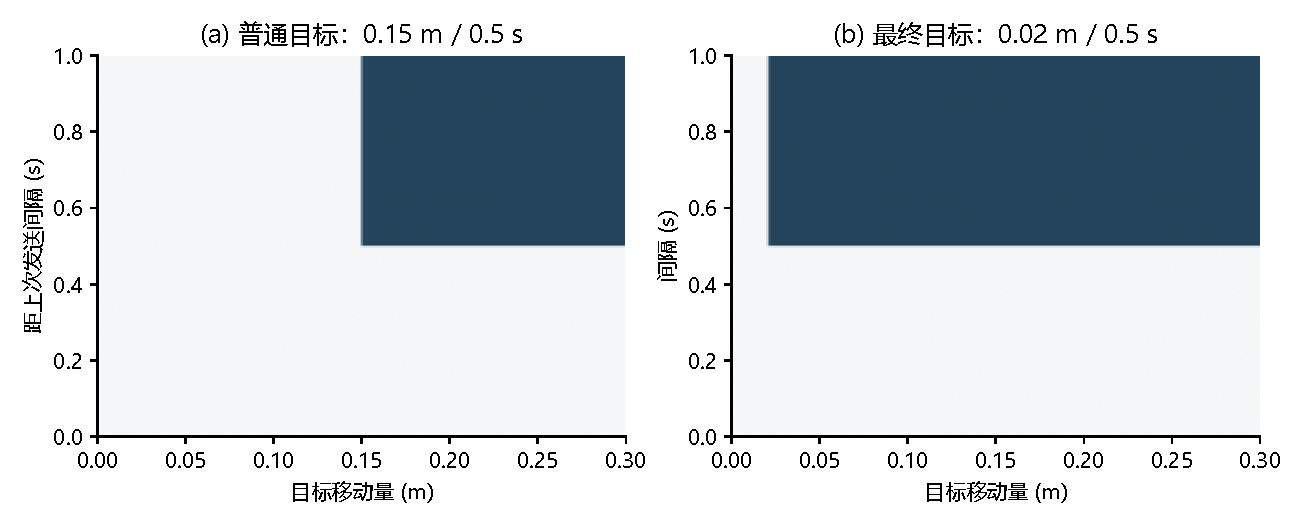
\includegraphics[width=.96\linewidth,height=85mm,keepaspectratio]{figures/analysis/goal_refresh.pdf}
\caption{实际 \texttt{need\_\allowbreak goal} 函数的普通/最终目标更新区域；与地图版本的 1 s/0.25 m 阈值区分使用。}\label{fig:f2a-goal_refresh}
\end{figure}

目标刷新同时约束发送时间与位置变化，目的是减少频繁抢占导航任务。其边界也意味着小幅移动可能不会产生新目标，因此终点停靠不能只依赖刷新触发。取消目标、任务许可与下游零速门控需要分别承担停止职责。

\begin{table}[H]\centering\small
\begin{tabularx}{\linewidth}{p{27mm}X}\toprule
核对项 & 技术含义与参数\\\midrule
限频收益 & 减少重复抢占和目标抖动\\
终点风险 & 目标移动小于阈值可能留在旧目标\\
停止路径 & 撤销许可 + \texttt{cancel\_\allowbreak goal} + 状态原因\\
\bottomrule\end{tabularx}
\caption{导航目标更新、取消与停止不变量的实现要点。}\end{table}

目标刷新解决导航输入变化，取消处理旧任务，门控零速约束实际底盘出口。三者的作用范围不同，实验记录应区分“停止发送新目标”“取消已有目标”和“速度已经降为零”，才能验证停止链是否完整。

\source{\path{turtlebot/follow2/multi_robot_following/scripts/map_follower.py}；\path{turtlebot/follow3/rgbd_following/src/rgbd_following_core/motion.py}。版本以本报告提交号及配置快照为准。}

\subsection{传感器观测与坐标一致性}
\subsubsection{Kinect深度到扫描：先验证观测再验证地图}
照片场地包含面板、立柱和较低障碍，二维导航所见范围由传感器视场、安装高度、俯仰和深度转扫描采样行共同决定。现场曾报告约35 cm障碍未稳定进入地图，应沿原始深度、转换后的scan、TF、地图四层排查。若原始深度没有有效返回，地图膨胀无法补造障碍；若深度有而scan没有，需核对采样高度、有效量程与相机姿态；若scan有而地图无，再检查TF、更新和清除配置。

二维LaserScan不是所有三维障碍的完整表示。把一段图像列的深度压缩到平面会丢失高度结构，过低采样可能遇到地面，过高采样可能越过低障碍。实验不能只按URDF的理想安装假定覆盖已满足。报告应保存深度与scan的同期截图、障碍实测高度、距离与相机安装，并按距离逐点检查有效性。
\begin{table}[H]\centering\small\begin{tabularx}{\linewidth}{p{28mm}YY}\toprule 检查层 & 观察内容 & 可定位的问题\\\midrule
原始深度 & 障碍ROI有效深度与缺测 & 反光、近距盲区、遮挡、驱动\\
转换扫描 & 同方向是否有合法range & 采样行、量程、安装俯仰\\
坐标变换 & optical到base与odom连通 & 外参、时间、硬编码frame\\
地图/代价层 & marking、clearing与高度范围 & 更新链、地图时效、清除覆盖\\\bottomrule\end{tabularx}\caption{35 cm障碍问题的分层定位顺序。}\end{table}

排查顺序从原始深度到扫描、代价地图，最后到速度出口，能够定位障碍信息在哪一层丢失。若原始传感器未覆盖目标，增大膨胀半径也无法恢复缺失观测；若地图已有障碍而车仍前进，则应检查规划和发布链。

\source{\code{docs/vm_follow2.md}；\code{latex/sections/30_follow2.tex}；课程传感器链配置。}

\subsubsection{地图版本、AMCL初值与长走廊可观测性}
赛道面板几何重复，长直通道中扫描对横向位置和朝向约束通常强于沿通道方向约束；转角、横板和不同间距提供更多几何区别。这是定位设计的几何分析，不是对当前AMCL误差已测得的结论。初始位姿应在实际地图上给定，随后检查激光与墙面重合、粒子分布和实际运动方向，而不是只看RViz中存在一簇粒子。

地图保存需要yaml与pgm成对，记录分辨率、原点、障碍版本和采集时刻。任何面板移动都可能改变原自由区；比赛前地图不应混用参考room地图或照片拓扑图。建图阶段结束要停止GMapping，再运行AMCL，保证map到odom唯一发布者。多台车共享map原点，但各车odom和base保持独立，不能仅在launch最外层加namespace就假定驱动内部frame也已经独立。
\source{\code{navigation.launch}；\code{localization_refresh.py}；\code{docs/interfaces.md}。}

\subsubsection{观测时间的TF变换及三类坐标误用}
AR位姿必须按实际采样时间变换到map，保留原始stamp。机器人在图像与最新TF之间可能已移动，如果用当前变换处理旧像素，目标会产生虚假位移；这种误差还会进入轨迹缓存，影响后续路径切线和间距。\texttt{marker\_\allowbreak target}没有有效TF时丢弃，不将旧观测重新包装成当前时间。
\begin{equation}
{}^m p_t(t_z)={}^mT_c(t_z)\,{}^cp_t(t_z),\qquad \delta p_{\perp}\approx z\,\delta\theta.
\end{equation}
三类误用尤其要避免：把optical的前向Z直接当base的高度Z；把前车独立odom数值当共享map位姿；把ALVAR标签姿态当人形行走朝向。前两者破坏空间一致性，后者可能让后退目标落到侧墙。当前方式二使用轨迹切线而非标签yaw，正确保留这个区分。
\source{\code{marker_target.py}；\code{pose_relay.py}；\code{map_follower.py}。}

\subsubsection{观测时间与变换时间的对应}
图\ref{fig:observation-time}将图像采样时刻和检测结果接收时刻分开。即使目标在世界中静止，本车在两时刻之间的位姿变化也会影响其相机坐标；正确变换需要查询采样时刻的相机位姿。图中仅表达时间先后，不假定具体传输延迟。
\begin{figure}[H]\centering
\resizebox{\linewidth}{!}{\begin{tikzpicture}[>=Stealth,font=\small]
\draw[->,Navy,thick] (0,0)--(14.2,0) node[right] {$t$};
\node[anchor=east,text=Navy] at (0,1.15) {视觉观测};
\node[anchor=east,text=Teal] at (0,-1.15) {位姿变换};
\fill[Navy] (2,0) circle (2pt);\fill[Navy] (10,0) circle (2pt);
\node[above,align=center,text=Navy] at (2,.25) {图像采样\\$t_z$};
\node[above,align=center,text=Navy] at (10,.25) {检测结果接收\\$t_r$};
\draw[<->,Muted] (2,-.4)--node[below,fill=white] {传输与识别延迟 $t_r-t_z$}(10,-.4);
\node[draw=Teal,fill=Teal!5,rounded corners=2pt,align=center,inner sep=2.5mm] (tf) at (2,-2) {查询 $T^{\rm map}_{\rm camera}(t_z)$\\保留观测原时间戳};
\node[draw=Rust,fill=Rust!5,rounded corners=2pt,align=center,inner sep=2.5mm] at (10,-2) {误用接收时刻 $t_r$\\可能把本车运动混入目标位移};
\draw[->,Teal] (2,-.65)--(tf.north);
\end{tikzpicture}
}
\caption{带时间戳的目标观测与 TF 查询关系。接收延迟不应改变观测所属时刻。}\label{fig:observation-time}
\end{figure}
将旧观测重新盖上当前时间戳会掩盖数据老化，并把机器人运动造成的坐标变化混入目标轨迹。反之，保留采样时间却缺少对应的 TF 历史也无法完成可靠变换，适配器应拒绝该样本。现场联调需同时检查设备时间同步、TF 缓存覆盖和图像消息时间戳，这三项分别约束时间基准、查询可达性与观测归属。
\source{\code{marker_target.py}：按标记时间戳查找 TF 并发布地图坐标目标。}

\subsection{控制架构与双层安全门控}
\subsubsection{ROS节点、话题和唯一速度发布链}
方式二的感知入口与导航执行通过\texttt{target\_\allowbreak pose}连接。\texttt{marker\_\allowbreak target}只适配目标坐标，不直接控制底盘；\texttt{map\_\allowbreak follower}检查任务、定位、地图、TF和间距后向\texttt{move\_\allowbreak base}发送目标并周期发布\texttt{motion\_\allowbreak allowed}。导航原始速度再进入独立\texttt{velocity\_\allowbreak gate}。图中分开任务桥、目标变换、规划和门控，有助于定位“看得见但不走”和“导航输出但被拒绝”的原因。
从控制责任看，\code{target_pose}只指定追踪对象的位置，导航器输出的是期望速度，\code{motion_allowed}则决定当前任务是否允许速度通过。后两者通过不同话题到达门控，必须同时满足条件，不能只因收到速度就放行。节点图因此将“目标”“速度”“许可”分别画成独立箭头，联调时需要逐条核对，尤其注意跨命名空间的重映射。

键盘遥控或其他直接发布者若仍连接同一底盘输入，会绕过门控；门控零速不能压制所有竞争源。联调要检查实际连接图、话题发布者和remap，关闭旧导航/遥控节点。多机情况下每车唯一输入、唯一frame前缀和共同时间基准应写入参数快照，而不是写死主机地址到共享文稿。

\begin{figure}[H]\centering\begin{tikzpicture}[box/.style={draw=Navy!65,line width=.8pt,rounded corners=3pt,fill=Navy!3,text width=35mm,minimum height=19mm,align=center,inner sep=3mm,font=\small,text=black},act/.style={box,draw=Teal,fill=Teal!6},warn/.style={box,draw=Rust,fill=Rust!6},edge/.style={-{Stealth[length=2.3mm]},line width=.9pt,draw=Navy},tag/.style={font=\footnotesize,text=Navy,fill=white,inner sep=1.3pt}]
\node[box] (ar) at (0,0) {\textbf{AR 目标检测}\\[1mm]\texttt{ar\_pose\_marker}};
\node[act] (tf) at (5.3,0) {\textbf{目标坐标适配}\\[1mm]\texttt{marker\_target} + TF};
\node[box] (mi) at (10.6,0) {\textbf{任务与定位状态}\\[1mm]任务桥 + AMCL};
\node[box] (f) at (5.3,-3.1) {\textbf{地图跟随器}\\[1mm]\texttt{map\_follower}};
\node[act] (nav) at (10.6,-3.1) {\textbf{全局／局部规划}\\[1mm]\texttt{move\_base} / DWA};
\node[warn] (ga) at (5.3,-6.2) {\textbf{独立速度门控}\\[1mm]\texttt{velocity\_gate}};
\node[box] (base) at (10.6,-6.2) {\textbf{底盘导航输入}\\[1mm]\texttt{cmd\_vel\_mux}};
\draw[edge] (ar)--node[tag,above] {测量时刻}(tf);
\draw[edge] (tf)--node[tag,right] {地图目标位置}(f);
\draw[edge] (mi.south west)--node[tag,above,sloped] {任务与定位有效性}(f.north east);
\draw[edge] (f)--node[tag,above] {导航目标}(nav);
\draw[edge] (f)--node[tag,left] {运动许可}(ga);
\draw[edge] (nav.south)--(10.6,-4.65)-|node[tag,pos=.25,above] {原始导航速度}([xshift=10mm]ga.north);
\draw[edge] (ga)--node[tag,above] {安全速度}(base);
\node[box,align=left] at (0,-3.1) {\textbf{职责区分}\\跟随器：目标与许可\\门控：安全速度出口};
\end{tikzpicture}
\caption{方式二节点与数据链。任务、定位与TF是导航许可条件，安全速度应只有一个最终出口。}\label{fig:f2-nodes}\end{figure}
图中的速度门控处于底盘导航输入之前，其安全作用依赖于实际话题连接和控制源唯一性。复现时应把这张逻辑图与真实 ROS 连接图对照，分别确认导航原始速度、运动许可和最终安全速度的发布者，而不是只检查节点是否启动。
\source{\code{follow_map.launch}；\code{navigation.launch}；\code{velocity_gate.py}。}

\subsubsection{地图跟随器的状态优先级与故障锁定}
\texttt{map\_\allowbreak follower}的step依次检查finished/failed、任务、目标、定位、地图、TF，然后检查当前最小间距、历史轨迹长度和目标足迹。较前的守卫失败就block并返回，所以多个问题同时发生时，\texttt{follow\_\allowbreak status}只显示先遇到的原因。实验应保存原始输入的有效性，不能从单个状态字符串断言其他层都正常。

地图版本将ABORTED、REJECTED、LOST锁为failed，需要排故后重启；目标暂失或地图过期则撤销许可和取消目标，等待有效输入恢复。finished则是任务done且接近后置点的简化完成条件，不包含RGB-D方案的完整终点多边形/停稳保持。报告不能将两套follower的结束功能混写，现场需补充进入终点并停稳的独立证据。
这组守卫构成逐层收缩的运动许可：上游确认目标与空间条件，下游独立确认命令、许可和扫描是否新鲜。任一环节通过都不意味着其他环节可以跳过，尤其不能用导航器内部避障替代命令看门狗。故障复现时应记录最先拒绝运动的守卫，避免把所有停车归因于规划失败。
\begin{figure}[H]\centering\begin{tikzpicture}[box/.style={draw=Navy!65,line width=.8pt,rounded corners=3pt,fill=Navy!3,text width=35mm,minimum height=19mm,align=center,inner sep=3mm,font=\small,text=black},act/.style={box,draw=Teal,fill=Teal!6},warn/.style={box,draw=Rust,fill=Rust!6},edge/.style={-{Stealth[length=2.3mm]},line width=.9pt,draw=Navy},tag/.style={font=\footnotesize,text=Navy,fill=white,inner sep=1.3pt}]
\node[box] (m) at (0,0) {\textbf{01\quad 任务与目标}\\[1mm]任务运行、目标有效};
\node[box] (l) at (5.3,0) {\textbf{02\quad 定位与坐标}\\[1mm]定位、地图、TF 有效};
\node[box] (p) at (10.6,0) {\textbf{03\quad 空间可行性}\\[1mm]间距、轨迹与足迹通过};
\node[act] (n) at (10.6,-3) {\textbf{04\quad 导航许可}\\[1mm]发送目标、导航未失败};
\node[warn] (g) at (5.3,-3) {\textbf{05\quad 速度安全复核}\\[1mm]时效、扇区距离与限速};
\node[act] (o) at (0,-3) {\textbf{06\quad 底盘安全输出}\\[1mm]通过则放行，否则零速};
\draw[edge] (m)--node[tag,above] {通过}(l);
\draw[edge] (l)--node[tag,above] {通过}(p);
\draw[edge] (p)--node[tag,right] {通过}(n);
\draw[edge] (n)--node[tag,above,align=center] {速度命令\\+ 许可}(g);
\draw[edge] (g)--node[tag,above] {复核结果}(o);
\node[draw=Rust!55,fill=Rust!4,rounded corners=2pt,text width=145mm,align=left,inner sep=3mm,font=\small,text=black] (failure) at (5.3,-5.5) {\textbf{失败处置分为两层}\\[1mm]上游条件失效：取消导航目标并撤销运动许可。\\下游复核不通过：独立门控输出零速，不依赖上游及时响应。};
\draw[edge,dashed,draw=Rust] (g.south)--(failure.north);
\end{tikzpicture}
\caption{方式二的分层守卫。任一上游条件失效取消目标，下游门控独立拒绝不新鲜命令。}\end{figure}

图中的安全输出只有在整条许可链成立时才放行；上游取消目标与下游零速是两个独立动作。故障日志应同时保存导航状态和门控原因，才能判断停车发生于哪一层。

\source{\code{map_follower.py}：step、block、stop。}

\subsubsection{扫描扇区、看门狗与缺测的保守解释}
Gate默认要求命令与许可各在0.4 s内刷新，扫描0.5 s内刷新。\texttt{scan\_\allowbreak clear}只保留量程内的有限样本，前方扇区至少三点且最小range大于停车距离才通过；NaN和Inf不能当成无障碍。直行时扇区为正负45度，转向角速度超过阈值时扩大到正负90度，仍不等于全车外围都有激光覆盖。

输出线程每0.05 s按墙钟运行，使ROS模拟时钟暂停时仍能归零。该看门狗使用接收时刻与测量时刻的共同约束，防止旧扫描迟到后被当作当前安全。拒绝倒车因为前方扫描不能证明后方空间安全；有限速度夹紧只限制命令，不证明硬件实际制动。地图与足迹检查、传感器覆盖和急停仍需分层验证。
左图把每种时效阈值的有效区间分行显示，负时间差与超过阈值的样本均应拒绝；右图给出车体半径对理想横向余量的影响。两者分别约束信息是否可信和空间是否足够，实际窄道通行还需扣除定位误差与障碍更新延迟造成的余量消耗。
\begin{figure}[H]\centering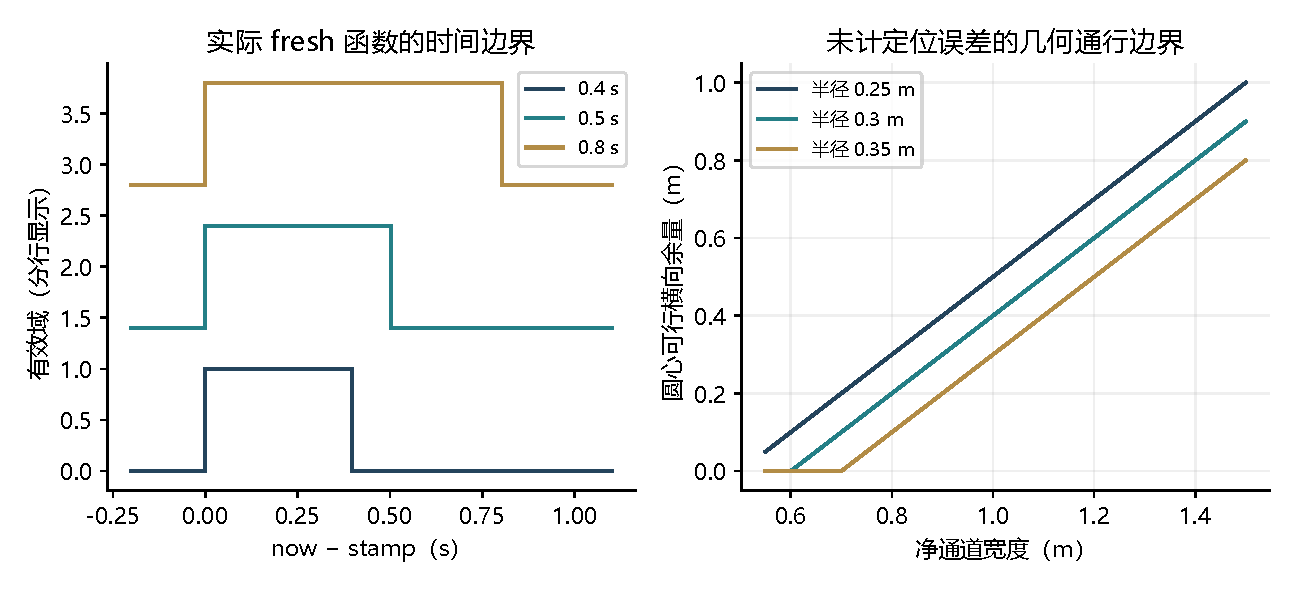
\includegraphics[width=\linewidth]{figures/analysis/fresh_clearance.pdf}\caption{fresh时间边界与通道几何余量。右图未计定位误差，是解析设计关系而非实测通行结果。}\end{figure}

通道几何中的零余量只是理想圆形模型的边界；实际车体突出部分、定位偏差与动态障碍均会使可用空间进一步缩小。时效曲线和几何曲线应分别用于检查时间契约与足迹配置，不能用其中一条替代另一项验证。

\source{\code{velocity_gate.py}；\code{competition_core/planning.py}：fresh、scan\_clear。}

\subsubsection{多级时效门限与停车责任}
不同信息源承担不同角色，源码没有为所有消息设置同一个超时。图\ref{fig:fresh-budget}把各门限并列：速度命令和许可需要更紧的刷新周期，地图和定位允许较长的信息年龄。该排序描述配置约束，不是测得的端到端停止延迟。
\begin{figure}[H]\centering
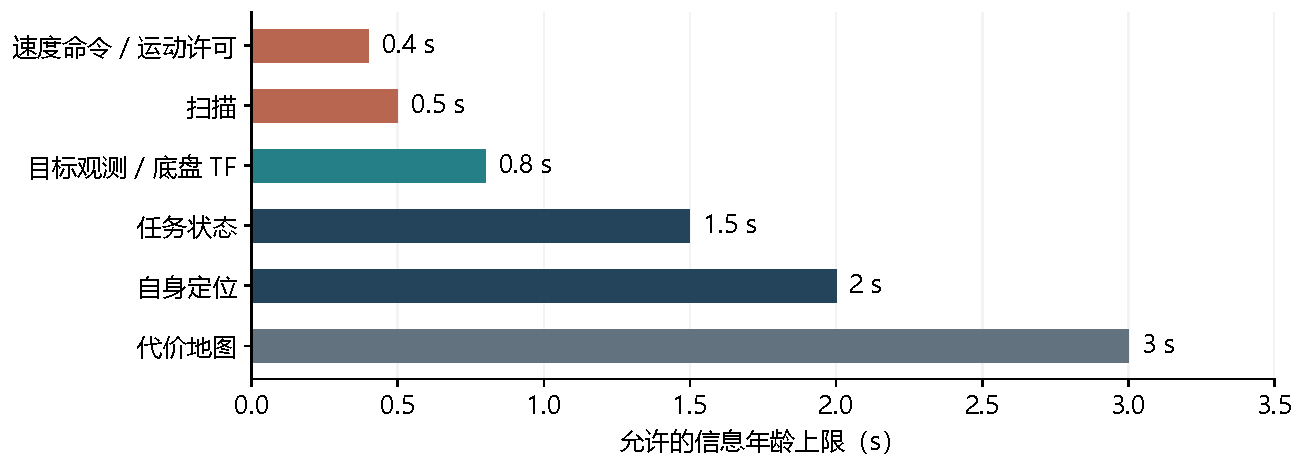
\includegraphics[width=.95\linewidth,height=.25\textheight,keepaspectratio]{figures/enriched/freshness_budget.pdf}
\caption{方式二关键输入的默认信息年龄上限。门控与跟随器分别采用各自时钟和检查逻辑。}\label{fig:fresh-budget}
\end{figure}
在链路失效时，停车首先由哪个条件触发取决于故障位置。目标消息中断可能由上游0.8\,s检查发现，许可或速度停止刷新则由下游0.4\,s看门狗拒绝；扫描缺失有独立0.5\,s约束。上述门限还需加上调度、传输和物理制动过程才能形成实际停止时间，不能把最短门限直接写为整机安全响应。

年龄检查也依赖时间语义。门控使用接收侧墙钟保持独立性；目标和 TF 则需要可比较的采样时间。若不同设备时钟存在偏移，简单放宽超时可能掩盖同步错误。应先确认时钟与数据更新契约，再结合运动速度和可用安全距离确定阈值。
\source{\code{map_follower.py}与\code{velocity_gate.py}。}

\subsubsection{窄道足迹、栅格补偿与参数耦合}
圆形足迹半径必须覆盖车身和突出结构，栅格检查额外补偿半格对角线。通道净宽w、半径r的理想横向余量为w减2r，但真实可用余量还需扣除定位、地图边界、传感器安装误差和动态侧摆。理论曲线只能帮助发现参数冲突，不能证明车在实际围挡中通过。
\begin{equation}
\Delta w_{\mathrm{usable}}\le w-2r-2\epsilon_{\mathrm{loc}}-2\epsilon_{\mathrm{map}},\qquad r_{\mathrm{check}}=r+\frac{\sqrt2}{2}s.
\end{equation}
跟随距离、目标更新阈值、速度上限、DWA预测时长和膨胀半径互相影响。增大间隔缓解追尾，却可能使目标在转角被遮挡；增大膨胀偏向通道中心，却可能使局部目标不可行；降速减小制动距离，但不修复未知或漏检障碍。调参应基于失败类别逐项调整，不把所有停车归结为“速度太低”。
\source{\code{costmap_common.yaml}；\code{move_base.yaml}；\code{planning.py}。}

\subsection{任务联动与实验评价}
\subsubsection{TonyPi最新入口与方式二的任务接口缺口}
通用competition.py能够发送UDP状态，\texttt{mission\_\allowbreak bridge}验证发送端、session、\texttt{run\_\allowbreak id}和递增sequence，缺数据超过1 s发布stopped。最新\texttt{marker\_\allowbreak route}是独立入口，尚未实现同一心跳。因此二者分别能运行不能证明自动协同完成，报告应把这一集成点明确画成待对接接口。

建议适配映射为：等待和暂停映射idle/stopped，实际抱物行走和转角映射carrying，释放映射releasing，正常结束映射done，异常映射fault。此处是接口设计建议，本次只改报告，不修改机器人控制代码，也不声称这些映射已经执行。映射还需明确持物是否确认、暂停是否立即撤销许可、done心跳持续多久，以及后车完成何时结束Pi进程。
\begin{table}[H]\centering\small\begin{tabularx}{\linewidth}{p{33mm}p{30mm}Y}\toprule 人形阶段 & 建议任务状态 & 对接要点\\\midrule
等待/暂停 & idle/stopped & 不允许后车继续运动\\
抱物行走/转角 & carrying & 持续心跳；身份与扫描仍独立检查\\
放置 & releasing & 允许后车完成尾部跟随\\
完成/异常 & done/fault & 正常收队与故障停车区分\\\bottomrule\end{tabularx}\caption{拟议适配契约，非当前最新入口已接入的实现声明。}\end{table}

适配完成后还需分别验证正常运行、主动暂停、异常退出及通信中断时的状态传播。只有领航任务状态能稳定触发跟随许可撤销，才能将该接口认定为联动功能，而非仅存在相同名字的话题。

\source{\code{mission_bridge.py}；\code{marker_route.py}；\code{competition.py}。}

\subsubsection{单车导航到移动目标的实验阶梯}
方式二验证顺序应是基础驱动、扫描覆盖、地图质量、静态定位、静态目标导航、动态AR目标、失效注入、再多车联调。这样可区分感知漏检和规划问题；35 cm障碍未确认之前直接多车穿行，会使失败原因混杂。各阶段以独立trial记录代码、参数、地图和视频索引。

静态目标先检查AMCL初值与目标可达性，再让TonyPi低速直行。左/右弯分别观察遮挡后停车、重捕获与目标轨迹连续性；移开标签测试目标话题静默，而不只测试检测器发空数组。停止任务、扫描或TF分别记录底盘实测停稳延迟。急停命令发出到门控零速，与零速命令到物理停止是两个时间，日志中应分别保留。
\source{\code{docs/vm_follow2.md}；\code{latex/data/experiment_records.csv}。}

\subsubsection{方式二结果的指标与失效归因}
报告同时记录欧氏间距误差和沿路径弧长间隔，拐角处两者不同；目标点沿折线后退并不证明底盘精确复现折线。应对比本车轨迹与领航历史路径的横向距离，结合最小障碍余量、丢失时长和暂停原因。DWA重规划可能在自由空间切角，此时区分目标生成、规划偏移和定位误差。
\begin{equation}
e_E(t)=\|p_r-p_l\|-d_f,\quad e_\perp(t)=\min_{q\in\Gamma_l}\|p_r-q\|,\quad T_{\mathrm{stop}}=t_{\mathrm{stopped}}-t_{\mathrm{fault}}.
\end{equation}
停止可能是任务许可暂停、目标丢失、间距过小、地图过期、足迹受阻或导航失败，含义不同。\texttt{waiting\_\allowbreak for\_\allowbreak leader\_\allowbreak trail}属于启动等待，不能与导航失败一概统计。当前没有完整实机日志，不填虚构成功率；既有Kinetic隔离检查只支持部分失效零速逻辑，并不证明物理避障或全程跟随成功。
\source{\code{map_follower.py}；\code{velocity_gate.py}；实验原始记录。}
